
\documentclass[10pt,twoside,slovak,a4paper]{article}

\usepackage[slovak]{babel}
%\usepackage[T1]{fontenc}
\usepackage[IL2]{fontenc} % lepšia sadzba písmena Ľ než v T1
\usepackage[utf8]{inputenc}
\usepackage{graphicx}
\usepackage{url} % príkaz \url na formátovanie URL
\usepackage{hyperref} % odkazy v texte budú aktívne (pri niektorých triedach dokumentov spôsobuje posun textu)

\usepackage{cite}
%\usepackage{times}

\pagestyle{headings}

\title{Článok} % meno a priezvisko vyučujúceho na cvičeniach

\author{Danylo Tokarskyi\\[2pt]
	{\small Slovenská technická univerzita v Bratislave}\\
	{\small Fakulta informatiky a informačných technológií}\\
	{\small \texttt{xtokarskyi@stuba.sk}}
	}

\date{\small 12. 10. 2022} 



\begin{document}

\maketitle

\begin{abstract}
\ldots
\end{abstract}



\section{UMLetino}
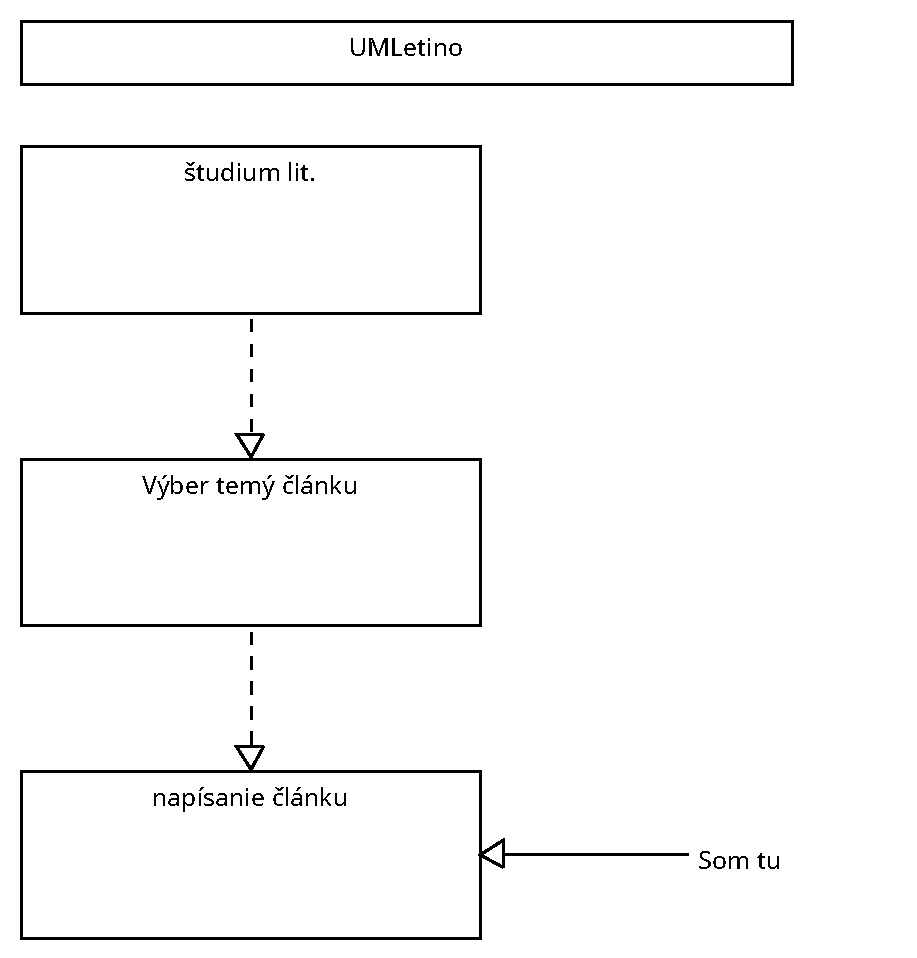
\includegraphics[scale=0.75,page=1]{umletino.pdf}

\section{GIMP}
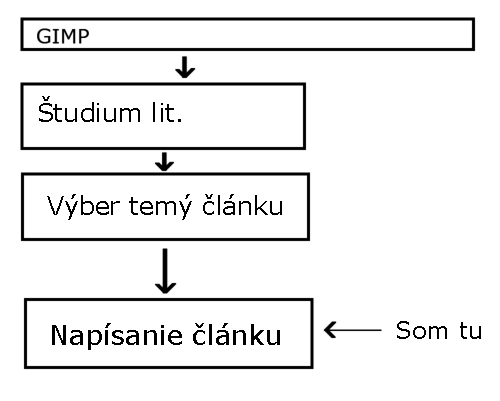
\includegraphics[scale=0.75,page=1]{gimp.pdf}






\bibliography{literatura}
\bibliographystyle{plain} % prípadne alpha, abbrv alebo hociktorý iný
\nocite{*}
\end{document}
